\chapter{Data Analysis}
As mentioned before, though of the fast helicity flipping and tremendous effort to keep 
the electron beam in exactly the same conditions through opposite helicity states, 
there is no way to achieve such a goal. There are always various noises produced
in various parts of the accelerator, though being very small in a general sense, 
they are large enough to flood what we are measuring, if not dealt with properly.  

We use the same methods to process both PREX-II and CREX data sets, therefore we will
discuss only CREX data here, anything that is different in PREX-II will be listed
out.

\begin{table}
    \centering
% with cut ErrorFlag&0xda7e6bff == 0 and minirun_size >= 4500
    \begin{tabular}{c | c}
	\hline
	Number of Good Slugs	    & 121   \\
	Number of Good Runs	    & 1384  \\
	Number of Good Miniruns	    & 8525  \\
	Number of Good Quadruplets  & 86832046  \\
	\hline
	Charge Asymmetry    & $\sim 100$~ppb	\\
	Position Difference & $\sim 10$~nm  \\
	Angle Difference    & $\sim 1$~nrad \\
	Energy Difference   & $\sim 10$~ppb \\
	\hline	    
	Raw Asymmetry	    & $2087$~ppm    \\
	Regressed Asymmetry & $2090$~ppm    \\
	\hline
    \end{tabular}
    \caption{CREX data statistics.}
\end{table}

% \begin{table}
%     \centering
%     \begin{tabular}{c | c c c}
% 	\hline
% 	Variable    & Regression    & Dithering	    & Lagrangian    \\
% 	\hline
% 	Slope	\\
% 	Correction (ppm)  \\
% 	\hline
%     \end{tabular}
% \end{table}

\begin{comment}
    % https://prex.jlab.org/DocDB/0000/000009/001/riordan_err_recommend-3.pdf
    \begin{itemize}
	\item (design) PREX-II statistical width: $\sim 120\ ppm @30Hz$
	\item (design) BCM resolution: $40\ ppm$
	\item (measured) 1 MHz BCM electronics: $\sim 25\ ppm @30 Hz, 20\ \mu A$
	\item charge and position jitter
	    $$ A_Q: 100-300\ ppm \quad \Delta x: 5-25\ \mu m$$
    \end{itemize}
\end{comment}

%%%%%%%%%%%%%%%%%%%%%%%%%%%%%%%%%%%%%%%%%%%%%%%%%%%%%%%%%%%%%%%%%%%%%%%%
\section{Raw Data}
CREX started commissioning around December 2019, we took the first good run on 
Dec 12. Six slugs (slug 100 - 105) were collected before the Christmas break. After 
the Christmas break, data taking was resumed until Jan 18 2020 when the first \Ca 
target was damaged. It took 5 days to prepare a new target.
Then things moved on quite smoothly, we had 2 days of transverse asymmetry (AT)
measurement from Feb 10 to Feb 12. We were a little over halfway on collected charge 
when Covid-19 hit and the lab was shut down at the end of March 2020. Fortunately,
the lab reopened four months later, we had the chance to continue the electron bombardment 
for another one month. The experiment stopped data taking on Sep 18 2020. A total charge
of 480~C was collected, among which 390~C was judged as good. 

The data set is clearly separated into three periods: before the AT, after the AT and before the Covid,
and after the Covid, in chronological order. 
A more reasonable split is to separate them by their wien-flip states, 
whose result almost overlaps with the chronological separation.

\begin{figure}[!h]
    \begin{tikzpicture}
	\begin{scope}
	    \node[anchor=south west, inner sep=0] (image) at (0, 0)
	    {   \includegraphics[width=0.45\linewidth]{charge_vs_time}
		\includegraphics[width=0.55\linewidth]{charge_vs_run} };
	    \begin{scope}[x={(image.south east)},y={(image.north west)}]
		\node [Violet] at (0.27, 0.8) {Covid-shutdown};
		\draw [-stealth, Violet, line width=1pt] (0.28, 0.75) -- (0.28, 0.6);
		\node [Violet] at (0.14, 0.65) {AT};
		\draw [-stealth, Violet, line width=1pt] (0.14, 0.61) -- (0.14, 0.3);
	    \end{scope}
	\end{scope}
    \end{tikzpicture}
    \caption{Charge accumulation versus time (left) and the run number (right). The
    long plateau on the left plot is due to the Covid shutdown, which is shown around
    run 7500 on the right plot. One sees that data taking is most efficient after
    the AT and before the Covid, the last month (after the Covid) is not bad while the 
    first two months are not so efficient due to various hardware problems.}
\end{figure}

CREX collects 1451 production runs, among them, 1386 are identified as `Good'
and used for final analysis. The good runs consists of 1362 both arms runs,
6 left arm runs and 18 right arm runs. Each good production run takes about 1~hour
and collects about 0.3~C with a charge efficiency of 80\%.
\begin{figure}[!h]
    \includegraphics[width=0.32\linewidth]{crex_run_time}
    \includegraphics[width=0.32\linewidth]{crex_run_charge}
    \includegraphics[width=0.32\linewidth]{crex_run_charge_efficiency}
    \caption{Runtime and charge statistics of CREX runs (\texttt{ErrorFlag == 0}).}
\end{figure}

Though electrons come bunch by bunch, the bunch frequency of 499~MHz is much
larger than our helicity flip frequency of 120~Hz, so electron beams can be regarded
as continous. All scattered electrons in one helicity window will be integrated as 1
readout (event). Every four continuous helicty events are grouped into one quadruplet
(in case of the 240~Hz flipping frequency in PREX-II, every eight helicity events 
form one octuplet).
In order to cancel the 60~Hz line power noise, the PV asymmetry is
calculated based on helicity quadruplets (octuplets in the case of 240~Hz flipping frequency), 
whose frequency will be 120/4 (230/8) = 30~Hz, as shown in Fig.~\ref{fig:helicity_pattern}. 
CREX collected about 87 million such good helicity quadruplets.
\begin{figure}[!h]
    \centering
    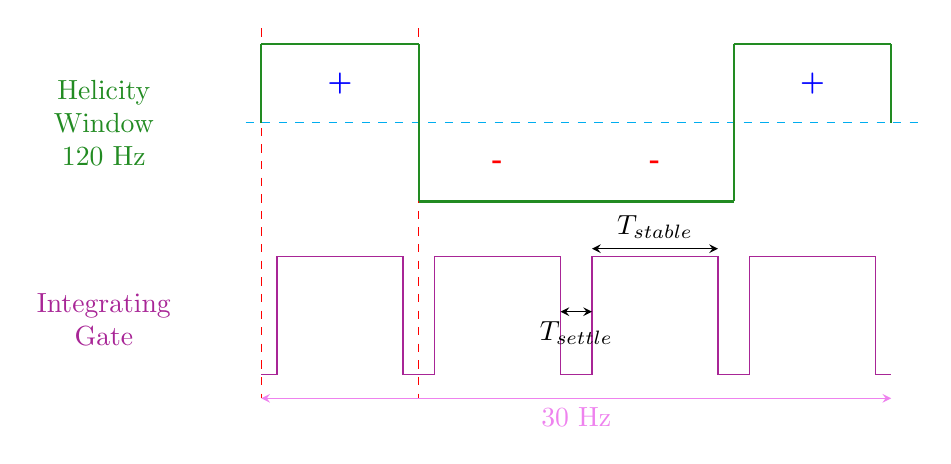
\begin{tikzpicture}[xscale=2]
	\tikzstyle{message} = [align = center]
	\draw[dashed, cyan] (-0.1, 0) -- (4.2, 0);
	\foreach \x in {0, 1}
	{ \draw[dashed, red] (\x, 1.2) -- (\x, -3.5); }
	\foreach \x in {0, 4}
	{ \draw[thick, ForestGreen] (\x, 0) -- (\x, 1); }
	\foreach \x in {1, 3}
	{ \draw[thick, ForestGreen] (\x, -1) -- (\x, 1); }
	\foreach \x in {0, 3}
	{ 
	    \draw[thick, ForestGreen] (\x, 1) -- +(1, 0); 
	    \node[blue] at (\x+0.5, 0.5) {\textbf{+}};
	}
	\foreach \x in {1, 2}
	{ 
	    \draw[thick, ForestGreen] (\x, -1) -- +(1, 0); 
	    \node[red] at (\x+0.5, -0.5) {\textbf{-}};
	}
	\node[message, ForestGreen, very thick] at (-1, 0) {Helicity \\  Window \\ 120 Hz};

	\foreach \x in {0, ..., 3}
	{
	    \draw[Mulberry] (\x, -3.2) -- ++(0.1, 0) -- ++(0, 1.5) -- ++(0.8, 0) 
	    -- ++(0, -1.5) -- ++(0.1, 0);
	}
	\draw[stealth-stealth, black] (2.1, -1.6) -- node[above] {$T_{\text{stable}}$}+(0.8, 0) ;
	\draw[stealth-stealth, black] (1.9, -2.4) -- node[below] {$T_{\text{settle}}$}+(0.2, 0) ;
	\draw[stealth-stealth, Violet] (0, -3.5) -- node[below] {30 Hz} +(4, 0);
	\node[message, Mulberry, very thick] at (-1, -2.5) {Integrating \\ Gate};
    \end{tikzpicture}
    \caption{Schematic plot of the helicity pattern. In CREX, $T_{\text{settle}} = 90\ \mu$s, 
    which allows the PC to stablize after a voltage polarity flipping, avoiding 
    any cross effect from the previous helicity state. The corresponding deputy factor 
    is 98.92\%.}
    \label{fig:helicity_pattern}
\end{figure}

\begin{figure}[!h]
    \centering
    \includegraphics[width=\linewidth]{run_6600_maindet}
    \caption{A run plot: detector yield and asymmetry distribution in run 6600, 
    selected with \texttt{ErrorFlag == 0}. The shift in the second half of the 
    yield plot is caused by the beam position/angle fluctuation. 
    The right 2 plots are average and difference of the asymmetry of LHRS and RHRS. 
    Ideally, the difference should be 0 and the average is what we want to measure.
    }
\end{figure}

Every run is separated into multiple miniruns to account for the fact that beam
conditions are changing quickly. It is inappropriate to calculate the detector
slope -- detector's response to the beam fluctuations, over a 60 mins time scale. 
Minirun will be more proper, the beam conditions, and therefore
the slope value should be more stable during such a shorter time period.  
Every minirun contains 9000 good quadruplets, which counts about 5~mins
in data collection. The last minirun in each run contains 
whatever number of good quadruplets left that can't be divided into 2 miniruns. 
Miniruns whose number of samples is less half of the standard (4500) will be discarded.
CREX has 8543 miniruns from 1386 good runs, among them, 2 miniruns are discarded
because of their small sample size and 16 miniruns are discarded due to noisy beam conditions 
or large beam shifts that are not caught in the previous two respins, as shown
in Table~\ref{tab:short_miniruns} and \ref{tab:bad_miniruns}.
To avoid another respin, these miniruns are simply removed. % which counts ??? C.
\begin{table}[!h]
    \centering
    \begin{tabular}{c c c}
	\hline
	run & minirun	& number of samples \\
	\hline
	% 5972	& 0 & 4385  \\
	% 6691	& 0 & 4080  \\
	7720	& 0 & 4352  \\
	8082	& 0 & 4391  \\
	\hline
    \end{tabular}
    \caption{Two miniruns that have too small good samples (with cut \texttt{ErrorFlag == 0}).}
    \label{tab:short_miniruns}
\end{table}
\begin{table}[!h]
% http://ace.phys.virginia.edu/HAPPEX/4606
    \centering
    \begin{tabular}{c c | c c}
	\hline
	run & minirun	& run	& minirun   \\
	\hline
	6564	& 4	& 7211	& 4 \\
	6567	& 2, 4	& 7889	& 0 \\
	6571	& 3, 4	& 7942	& 5 \\
	6593	& 2	& 8036	& 2 \\
	6983	& 8	& 8240	& 1 \\
	7149	& 6	& 8549	& 0, 1, 4   \\
	\hline
    \end{tabular}
    \caption{List of Miniruns that had larger asymmetry outliers and therefore
    are removed.}
    \label{tab:bad_miniruns}
\end{table}
\begin{figure}[!h]
    \centering
    \includegraphics[width=\linewidth]{run_6620_mini_asym_us_avg.mean}
    \caption{A minirun plot: mean values of asym\_us\_avg of each minirun in 
    run 6620 (\texttt{ErrorFlag == 0}).
    The red line is a zero-order polynomial fit and the bottom histogram is
    the ratio of the deviation to the mean fit value w.r.t. each point's uncertainty.
    }
\end{figure}

Runs will be grouped into slugs. One slug is defined as all runs between two
changes of the IHWP. With a stable beam, we could collect three slugs per day, so 
each slug takes about 8~hours or longer in case of any accidents. CREX collectes
124 slugs, after the data cleaning and combination to remove slugs with only 1 run, 
121 slugs are kept.
% slug 100 - 223
% slug 105, 117 and 123 are removed
\begin{figure}[!h]
    \centering
    \includegraphics[width=\linewidth]{slug_150_asym_us_avg.mean}
    \caption{A slug plot: minirun-wise distribution of asym\_us\_avg in slug 150 
    (\texttt{ErrorFlag == 0}).}
\end{figure}

Finally, slugs are split into periods, with different wien flip states. 
We have three periods as said before.
\begin{table}[!h]
    \centering
    \begin{tabular}{c | c}
	\hline
	wien-flip   & slugs \\
	\hline
	Right	& 100-137   \\
	Left	& 138-185   \\
	Right	& 186-223   \\
	\hline
    \end{tabular}
    \caption{Wien-flip separation in terms of slugs.}
\end{table}

%%%%%%%%%%%%%%%%%%%%%%%%%%%%%%%%%%%%%%%%%%%%%%%%
\subsection{Cut}
A loose cut is applied in the event level to select as much as possible good events.
During data taking, the JAPAN analyzer will check various hardware failures, the
beam stability level, helicity information and others. Based on the total 23 checks,
an error code (ErrorFlag), which is the bit-wise OR of the result against every
check, is assigned to each event. Events that pass every check will have
a null error code (ErrorFlag == 0). 

The various hardware failure checks detects the ADC readout in the detectors and
monitors, making sure we are not recording saturation or null values; the 
sample size is also verified. These checks help to identify the problematic
hardware channels in case of any hardware failures.

The beam stability level checks keep track of the beam conditions based on their
mean and RMS values. These checks compare the detector/monitor readout to 
a user-set upper and lower limit to filter out outliers; besides, for some ADC 
channels, there are cuts on the RMS of a moving time window of 200 (configurable) % prex_ring_stability.xxxx.conf
consecutive events, if the RMS value is too large, 
all events in that time window fail the RMS check. 
Finally, the burplevel check compares the current event readout with the average
value of the previous 10 (configurable) events, events with difference larger than
the burplevel cut fail this check. With these checks, we can make sure the good 
quality of the data we collect.

One example of such stability cut is the beam current cut. In case of beam trip
due to various accidents, the beam drops and then recovers quickly. The beam in
the process of falling and rising is usually unstable, so we require the event
beam current should be larger than the stable beam current minus $30\ \mu$A ($15\ \mu$A in PREX-II).

\begin{figure}[!h]
    \centering
    \includegraphics[width=\linewidth]{8019_bpm4aX}
    % \includegraphics[scale=0.28]{8019_bpm4aY}
    \caption{BPM4aX distribution (top) in run 8019, the bottom plot is the corresponding
    beam current distribution. Black points are good events (\texttt{ErrorFlag == 0}) 
    and red points are bad ones (\texttt{ErrorFlag != 0}). 
    One can clearly see that all beam trips and most beam jitters are recognized 
    by our stability checks.}
\end{figure}

Apart from these checks, we have an analysis shift worker to check monitor/detector 
yields and their differences/asymmetries for each run after prompting. Additional
cuts can be applied if large beam excursion, drift or any other anomalies are observed. 
These cuts are run specific, added one by one when needed.

During the online and the two offline analysis, we uses cut \verb|ErrorFlag == 0|
to select good quadruplets, which excluded all beam modulation events. Actually, 
some beam modulation events are usable for our asymmetry analysis and are
included in our final published result, which counts for about 5\% of the CREX data set.
To be consistent with the published result, all following plots are produced with the cut 
\verb|ErrorFlag&0xda7e6bff == 0| if not mentioned otherwise. 

%%%%%%%%%%%%%%%%%%%%%%%%%%%%%%%%%%%%%%%%%%%%%%%%
\subsection{Beam Conditions}
As explained before, the key to measure a teeny tiny asymmetry value is to 
keep all experimental conditions as the same as possible between different 
helicity windows. Among all the conditions that need precise control, the 
hardest one is the beam condition. Any fluctuation in any component along the 
long accelerator line will cause changes to the beam condition, therefore introducing false 
asymmetry to our measurement. Despite various difficulties, the CEBAF staff worked 
hard to provide us excellent beams with tiny difference between different helicity 
windows, as displayed below.

%%%%%%%%%%%%%%%%%%%%%%%%
\subsubsection{Beam Current}
The raw asymmetry we measure is normalized to the beam current, because beam
current varied from run to run; and even within a single run, beam currents are 
slightly different between helicity windows. The normalized raw asymmetry is:
\begin{equation}
    \CA_{\text{raw}} = \frac{(D/I)^+ - (D/I)^-}{(D/I)^+ + (D/I)^-}
	\approx \frac{D^+ - D^-}{D^+ + D^-} - \frac{I^+ - I^-}{I^+ + I^-}
	= \CA_D - \CA_I
\end{equation}
where D represents a detector readout.

This equation shows that the charge asymmetry contributes to the raw asymmetry directly, 
so we need to keep the charge asymmetry as small as possible, which is done 
through the charge feedback system. Overall, charge asymmetry is about hundreds of ppb. 
One can also tell from Fig.~\ref{fig:crex_bcm_target}
that period 2 has relatively good beam conditions than the other two periods.
\begin{figure}[H]
    \centering
    \includegraphics[width=0.32\linewidth]{crex_yield_bcm_target.mean}
    \includegraphics[width=0.32\linewidth]{crex_asym_bcm_target.mean}
    \includegraphics[width=0.32\linewidth]{crex_reg_asym_bcm_target.mean}
    \caption{Slug-wise mean value of the beam current, asymmetry and regressed 
    asymmetry in CREX (\texttt{ErrorFlag == 0}). The blue dashed lines separate
    the data set into three periods with different wien-flip states.
    Most of the time, CREX run at $\sim 150\ \mu$A, an overall $\sim 100~$~ppb charge 
    asymmetry is achieved.}
    \label{fig:crex_bcm_target}
\end{figure}

%%%%%%%%%%%%%%%%%%%%%%%%
\subsubsection{Beam Position, Angle and Energy}
% target position/angle oscillation: http://ace.phys.virginia.edu/HAPPEX/4520
We don't have a direct measurement of the beam position and angle at the target, these 
information can be inferred from various BPMs. Given the 
distance between the target and BPM4a as $D1 = 5.725$~m and the distance
between BPM4a and BPM4e as $D2 =4.083$~m, the beam position and angle at the target 
will be:
\begin{equation}
    \begin{aligned}
	T_{X,Y} &= \text{BPM4a}_{X,Y} + \frac{\text{BPM4e}_{X,Y} - \text{BPM4a}_{X,Y}}{D2} D1	\\
	\theta_{X,Y} &= \frac{\text{BPM4e}_{X,Y} - \text{BPM4a}_{X,Y}}{D2} \\
    \end{aligned}
    \label{eq:target_pos}
\end{equation}
Using Eq.~\ref{eq:target_pos}, the overall difference of the beam position/angle 
at the target is calculated to be:
\begin{equation*}
    \text{diff}_{X,Y} \sim 10\ \mathrm{nm}	\qquad \text{diff}_{\theta_{X,Y}} \sim \mathrm{nrad}	
\end{equation*}
Again, the second period has a more stable beam than the other two periods.

\begin{figure}[!h]
    \centering
    \includegraphics[width=0.49\linewidth]{crex_diff_targetX.mean}
    \includegraphics[width=0.49\linewidth]{crex_diff_thetaX.mean}
    \caption{Slug-wise mean value of the beam position (left) and angle (right) 
    difference at the target. 
    Very precise control of the beam conditions is achieved.
    The Y dimension plots are similar and are not shown here.}
\end{figure}

The beam momentum/energy is measured by BPM12X, whose dispersion tells the deviation
(dp) from the standard value (p0). The design value of the dispersion for CREX is
$D = 4.0$~m, and an actual measurement gives $\sim3.8$~m. I use 4.0~m here.
As can be seen in Fig.~\ref{fig:crex_diff_p}, CEBAF provides a beam with energy 
dispersion as small as $\sim10$~ppb.

\begin{equation}
    \frac{dp}{p} = \frac{\text{diff\_BPM12X}}{D}
\end{equation}

\begin{figure}[!h]
    \centering
    \includegraphics[width=0.6\linewidth]{crex_diff_p.mean}
    \caption{Slug-wise mean value of the beam energy dispersion. Overall, 
    an energy difference of $\sim 10$~ppb is achieved. }
    \label{fig:crex_diff_p}
\end{figure}

%%%%%%%%%%%%%%%%%%%%%%%%%%%%%%%%%%%%%%%%%%%%%%%%
\subsection{Raw Asymmetry}
% pedestal correction
The raw asymmetry is calculated as:
\begin{equation}
    \CA_{\text{raw}} \equiv 
    \begin{cases}
	\frac{d^+ - d^- - d^- + d^+}{d^+ + d^- + d^- + d^+}	& (+--+\ \text{pattern})    \\
	\frac{-d^- + d^+ + d^+ - d^-}{d^+ + d^- + d^- + d^+}	& (-++-\ \text{pattern})    \\
    \end{cases}
\end{equation}
where $d=\frac{D}{I}$ is the normalized detector integrating yield in one helicity
window, the upper-script indicate the helicity of the beam. The detector yield is
calibrated with their corresponding pedestals. 
% The raw asymmetry was blinded before final result was freezed.
\begin{figure}[!h]
    \centering
    \includegraphics[width=0.49\linewidth]{crex_asym_us_avg}
    \includegraphics[width=0.49\linewidth]{crex_asym_us_dd}
    \caption{Slug-wise raw asymmetry average (left) and difference (right) for CREX. 
    The right plot has three less slugs because there are three single-arm slugs.}
\end{figure}

\begin{figure}[!h]
    \centering
    \includegraphics[width=0.49\linewidth]{crex_mulplot_asym_us_avg}
    \includegraphics[width=0.49\linewidth]{crex_mulplot_asym_us_dd}
    \caption{Mulplot of the CREX raw asymmetry average (left) and difference (right). 
    The blue line is the data and the red line is a Gaussian fit. 
    The difference plot has less entries because single arm runs have no difference.}
\end{figure}


%%%%%%%%%%%%%%%%%%%%%%%%%%%%%%%%%%%%%%%%%%%%%%%%%%%%%%%%%%%%%%%%%%%%%%%%
\section{Beam False Asymmetry Correction}
As shown in the previous few plots about beam conditions, there are false
asymmetries caused by the beam. The helicity correlated beam asymmetry (HCBA), 
is the largest contributor to the false asymmetry.

As one may notice in Fig.~\ref{fig:correlation}, a beam jitter will cause 
fluctuation in the detector yield, with approximately a linear correlation.
So to remove the false asymmetries caused by beam jitters, we just need to
know the correlation between the detector yield and each beam parameter -- 
the detector slope. 

\begin{figure}[!h]
    \centering
    \includegraphics[width=0.6\linewidth]{run7679_correlation}
    \caption{Correlation between the detector yield and the beam position/energy in run 7679.
    The left/right detector yields change oppositely when the beam position shifts,
    and they move in the same direction w.r.t. fluctuations in the beam energy.
    }
    \label{fig:correlation}
\end{figure}

There are 2 methods to calculate the slope value, regression and beam modulation,
we will discuss them in details in the following sections.

%%%%%%%%%%%%%%%%%%%%%%%%%%%%%%%%%%%%%%%%%%%%%%%%
\subsection{Regression}

The first method to calculate the slope is the regression -- a perfect scheme for
the application of this statistical tool.

Bear in mind that regression itself doesn't tell us any relationships or rules, 
it only works under
the assumption that the relationship between variables is predictable (given by the user) 
and the dependent variables follow a known distribution function $P(\epsilon)$, which,
again, will be told by the user:
$$ Y = f(X) + \epsilon $$
With these prior knowledge, regression is able to extract the most likely 
coefficients in the predicted model.

\begin{comment}
For example, the famous least square fit is actually a linear regression 
$$ Y = c_0 + \sum c_i x_i + \epsilon $$
assuming Gaussian distribution of the dependent variable: $\epsilon \sim N(0, \sigma)$
Another frequenctly used scene is logistic regression for classification, which
is very similar to linear regression except f(X) will be converted into a
probability function, e.g. using the logistic function:
$$ h(z) = \frac{e^z}{1 + e^z} \quad z = f(X) $$

The assumpsion we made here is that the fluctuations in beam parameters in small, 
compared to their normal yield -- this can be verified by their yield plot. So
that we can use first order fit to model the detector's response to change in
beam parameters. Therefore the `true' asymmetry will be:
\begin{equation}
    \CA_{cor} = \CA_{raw} - \sum_i \beta_i\Delta M_i
\end{equation}
where $\CA_{cor}$ is the corrected asymmetry, $\beta_i = \frac{\partial \CA_{raw}}{\Delta M_i}$ 
is the slope and $\Delta M$ is the difference of BPM yield bewtween 
opposite helicities windows, i sums over all 5 chosen BPMs.
\end{comment}

%%%%%%%%%%%%%%%%%%%%%%%%
\subsubsection{The Model}
Considering one monitor and one detector. Assuming the reading noise of the detector
follows the Gaussian distribution and the monitor is precise (one can absorb the monitor
noise into the beam fluctuation):
\begin{equation}
    \begin{gathered}
	M = m	\\
	D = d + \epsilon(0, \sigma_0^D)    \\
    \end{gathered}
\end{equation}
here, the capital letters (D and M) represent the measured values while the 
small letter (m and d) mean the true values. $\sigma_0^D$ 
is the variance of the noise in the detector.

Then the difference between beams of opposite polarization will follow also
the Gaussian distribution with a larger variance:
\begin{equation}
    \begin{gathered}
	\Delta M = M^+ - M^- = m^+ - m^- = \Delta m   \\
	\Delta D = D^+ - D^- = (d^+ + \epsilon(0, \sigma_0^D)) - (d^- + \epsilon(0, \sigma_0^D))
	    = \Delta d_0 + \epsilon(0, \sqrt{2}\sigma_0^D)
	    = \Delta d + \epsilon(0, \sigma_1^D) \\
    \end{gathered}
\end{equation}
Again, $\Delta m$ and $\Delta d$ are the real differences
while $\Delta M$ and $\Delta D$ are the measured values.

The probability for measuring $\Delta D$ will be:
\begin{equation}
    \begin{gathered}
	P(\Delta D) = \frac{1}{\sigma_1^D\sqrt{2\pi}} e^{-\frac{1}{2}\left( \frac{\Delta D - \Delta d}{\sigma_1^D}\right)^2}    \\
    \end{gathered}
\end{equation}

We will have a bunch of independent data points: $(\Delta M, \Delta D)_i$ and 
we want to extract the relationship between $\Delta d$ and $\Delta m$: 
$\beta \equiv \frac{\partial d}{\partial m}$. Given the tininess of $\Delta m$ (
compared to its normal yield), a first order correlation is precise enough. 
This is exactly a linear regression problem.
\begin{equation}
    \begin{gathered}
	\Delta d = 0 + \beta \Delta m	\\
	\CA_{\text{cor}} = \CA_{\text{raw}} - \beta\Delta M	\\
    \end{gathered}
    \label{eq:first_order_correlation}
\end{equation}
where $\CA_{\text{cor}}$ is the corrected asymmetry.

For any real data point $(\Delta m, \Delta d)_i$, the possibility to measure
$(\Delta M, \Delta D)_i$ is:
\begin{equation}
    \begin{gathered}
	P_i(\Delta D|\Delta M) = \frac{1}{\sigma_1^D\sqrt{2\pi}} 
	    e^{-\frac{1}{2}\left( \frac{\Delta D - \beta\Delta M}{\sigma_1^D}\right)^2}
    \end{gathered}
\end{equation}

For the accumulated data of one minirun, the total probability will be:
\begin{equation}
    P = \prod_i^n P_i(\Delta D|\Delta M) = \prod_i^n \frac{1}{\sigma_1^D\sqrt{2\pi}} 
	    e^{-\frac{1}{2}\left( \frac{\Delta D_i - \beta\Delta M_i}{\sigma_1^D}\right)^2}
\end{equation}

To maximize P, it is equivalently to minimize:
\begin{equation}
    \chi^2 = \sum_i (\Delta D - \beta\Delta M)_i^2
    \label{eq:regression_chi2}
\end{equation}
where i sums over all samples in one minirun.

Maximization of P w.r.t. $\beta$ means a zero derivative:
\begin{equation}
    \frac{\partial P}{\partial \beta} = P \times 
    \sum_i \frac{\Delta M_i}{\sigma_1^D} \left( \frac{\Delta D_i - \beta\Delta M_i}{\sigma_1^D}\right)
    = 0
\end{equation}
which gives $\beta$ as:
\begin{equation}
    \sum_i \Delta M_i (\Delta D_i - \beta\Delta M_i) = 0 
\end{equation}
$$ \Downarrow $$
\begin{equation}
    \beta = \frac{\sum \Delta D_i \Delta M_i}{\sum \Delta M^2_i}
\end{equation}

Extending the independent variable to be multi-dimensional, we have:
\begin{equation}
    \Delta D = \begin{pmatrix} \beta_1 & \beta_2 & \cdots & \beta_m \end{pmatrix} 
	\begin{pmatrix}
	    \Delta M^1	\\
	    \Delta M^2	\\
	    \vdots 	\\
	    \Delta M^m	\\
	\end{pmatrix}
	+ \epsilon(0, \sigma^D)
\end{equation}
where m is the number of BPMs used for the asymmetry analysis.
\begin{equation}
    \frac{\partial P}{\partial \beta_\nu} \propto \sum_i \Delta M_i^\nu (\Delta D_i - \sum_\mu \beta_\mu M_i^\mu) = 0
    \label{eq:mul_dim_derivative}
\end{equation}
Arrange Eq.~\ref{eq:mul_dim_derivative} in a matrix:
\begin{equation}
    \small
    \begin{pmatrix}
	\sum_i \Delta D_i \Delta M_i^1 \\
	\sum_i \Delta D_i \Delta M_i^2 \\
	\vdots	\\
	\sum_i \Delta D_i \Delta M_i^m \\
    \end{pmatrix}
    = 
    \begin{pmatrix}
	\sum_i \Delta M_i^1 \Delta M_i^1    & \sum_i \Delta M_i^1 \Delta M_i^2	&
	\cdots	& \sum_i \Delta M_i^1 \Delta M_i^m  \\
	\sum_i \Delta M_i^2 \Delta M_i^1    & \sum_i \Delta M_i^2 \Delta M_i^2	&
	\cdots	& \sum_i \Delta M_i^2 \Delta M_i^m  \\
	\vdots	& \vdots    & \ddots	& \vdots    \\
	\sum_i \Delta M_i^m \Delta M_i^1    & \sum_i \Delta M_i^m \Delta M_i^2	&
	\cdots	& \sum_i \Delta M_i^m \Delta M_i^m  \\
    \end{pmatrix}
    \begin{pmatrix}
	\beta_1 \\
	\beta_2 \\
	\vdots	\\
	\beta_m \\ 
    \end{pmatrix}
\end{equation}

Define the covariance of any two variables as:
\begin{equation}
    \text{cov}(x, y) = \sum_i x_i y_i
\end{equation}
and
\begin{equation}
    M_{m \times m} = 
    \begin{pmatrix}
	\text{cov}(\Delta M^1, \Delta M^1) & \text{cov}(\Delta M^1, \Delta M^2)   & \cdots & \text{cov}(\Delta M^1, \Delta M^m)  \\
	\text{cov}(\Delta M^2, \Delta M^1) & \text{cov}(\Delta M^2, \Delta M^2)   & \cdots & \text{cov}(\Delta M^2, \Delta M^2)  \\
	\vdots	& \vdots    & \ddots	& \vdots    \\
	\text{cov}(\Delta M^m, \Delta M^1) & \text{cov}(\Delta M^m, \Delta M^2)   & \cdots & \text{cov}(\Delta M^m, \Delta M^m)  \\
    \end{pmatrix}
    \label{eq:M_definition}
\end{equation}

The coefficient vector will be extracted as:
\begin{equation}
    \begin{pmatrix}
	\beta_1 \\
	\beta_2 \\
	\vdots	\\
	\beta_m \\ 
    \end{pmatrix}
    =
    M^{-1}
    \begin{pmatrix}
	\text{cov}(\Delta D, \Delta M^1)   \\
	\text{cov}(\Delta D, \Delta M^2)   \\
	\vdots	\\
	\text{cov}(\Delta D, \Delta M^m)   \\
    \end{pmatrix}
    \label{eq:slope}
\end{equation}

\begin{comment}
For multiple detectors, it is easy to get:
\begin{equation}
    \small
    \begin{aligned}
	\begin{pmatrix}
	    \beta_{11}	& \beta_{21}    & \cdots & \beta_{m1}	\\
	    \beta_{12}	& \beta_{22}    & \cdots & \beta_{m2}	\\
	    \vdots	& \vdots    & \ddots	& \vdots\\
	    \beta_{1n}	& \beta_{2n}    & \cdots & \beta_{mn}	\\
	\end{pmatrix}
	&= A^{-1}
	&\times
	\begin{pmatrix}
	    \text{cov}(\Delta D^1, \Delta M^1) & \text{cov}(\Delta D^2, \Delta M^1)   & \cdots	& \text{cov}(\Delta D^m, \Delta M^1)	\\
	    \text{cov}(\Delta D^1, \Delta M^2) & \text{cov}(\Delta D^2, \Delta M^2)   & \cdots	& \text{cov}(\Delta D^m, \Delta M^2)	\\
	    \vdots	& \vdots    & \ddots	& \vdots    \\
	    \text{cov}(\Delta D^1, \Delta M^n) & \text{cov}(\Delta D^2, \Delta M^n)   & \cdots	& \text{cov}(\Delta D^m, \Delta M^n)	\\
	\end{pmatrix}
    \end{aligned}
    \label{eq:slope}
\end{equation}
where $\beta_{ij}$ refers to detector i's response to change in monitor j.
\end{comment}

Theoretically and practically, we need only 5 BPMs to cover the whole phase space of 
the beam motion.
The 5 BPMs we chose in CREX analysis are BPM1X, BPM4aY, BPM4eX, BPM4eY and BPM12X.

%%%%%%%%%%%%%%%%%%%%%%%%
\subsubsection{Slope Values}
With Eq.~\ref{eq:slope}, the slope values w.r.t. to the chosen BPMs are calculated. 
Fig.~\ref{fig:slug_202_reg_asym_us_avg_diff_bpm12X} shows the asymmetry's response
to changes in the beam energy, it justifies the usage of miniruns. 
As one can see in the plot, miniruns within the same run may have different 
slope values up to a few percent. This is expected because the detector slope 
is not a constant, it depends on the detector yield. 
Remember Eq.~\ref{eq:first_order_correlation} is based on the assumption that 
the beam fluctuations are tiny. When there are relatively large shifts in the 
beam, new slopes are needed. Therefore, a minirun-wise slope value is 
more stable than a run-wise one, and corrects the false asymmetry more precisely. 
This also means that the regression correction can deal with only small fluctuation 
around the mean value, it is imprecise to do the same correction for outliers, that's why
we need to remove miniruns with beam condition outliers.
\begin{figure}[!h]
    \centering
    \includegraphics[width=\linewidth]{slug_202_reg_asym_us_avg_diff_bpm12X}
    \caption{Minirun-wise energy slope ($\partial$(asymmetry average)/$\partial$ (BPM12X)) 
    distribution in slug 202. The X-axis is the run number attached by a minirun number.}
    \label{fig:slug_202_reg_asym_us_avg_diff_bpm12X}
\end{figure}

Table~\ref{tab:crex_slope} summarise the approximative slope values w.r.t. the 5
five BPMs we chose. Overall, our detector is sensitive to fluctuations in the X direction
(the disperse direction) and the beam energy, and is dull to jitters in the Y direction.
\begin{table}[!h]
    \centering
    \begin{tabular}{c | c}
	\hline
	BPM & slope (ppm/$\mu$m)   \\
	\hline
	1X  & $\sim -40$    \\
	4aY & $\sim 15$    \\
	4eX & $\sim 40$	\\
	4eY & $\sim 0$	\\
	12X & $\sim -40$    \\
	\hline
    \end{tabular}
    \caption{Slope values of the asymmetry average w.r.t. different BPMs.}
    \label{tab:crex_slope}
\end{table}

%%%%%%%%%%%%%%%%%%%%%%%%
\subsubsection{Corrections}
With the slope values, we can calculate the corresponding false asymmetry correction:
\begin{equation}
    \CA_{\text{false}} = \beta \times \text{(diff in BPM)}
\end{equation}
The main correction comes from differences in the X direction and the energy.
A typical correction is about a few ppm, as shown in Fig.~\ref{fig:slug_202_reg_asym_us_avg_diff_bpm12X}.
Due to detector's insensitivity to fluctuations in the Y direction, its correction 
is relatively small, at the level of  a few hundred ppb. Note that corrections
from each beam parameter don't add up, they actually cancel with each other,
leaving a relatively small total correction, usually a few ppm.

\begin{figure}[H]
    \centering
    \includegraphics[width=\linewidth]{slug_202_reg_asym_us_avg_diff_bpm12X_cor.mean}
    \caption{False asymmetry corection caused by the energy difference (BPM12X) in
    slug 202.}
    \label{fig:slug_202_reg_asym_us_avg_diff_bpm12X_cor}
\end{figure}

\begin{table}[!h]
    \centering
    \begin{tabular}{c | c}
	\hline
	BPM  & correction   \\
	\hline
	1X  & a few tenths ppm \\
	4aY & a few hundreds ppb     \\
	4eX & a few tenths ppm \\
	4eY & a few hundreds ppb     \\
	12X  & a few tenths ppm \\
	\hline
    \end{tabular}
    \caption{Typical false asymmetry corections from each BPM.}
\end{table}

%%%%%%%%%%%%%%%%%%%%%%%%
\subsubsection{Regression Result}
The asymmetry after the regression correction reads $2080 \pm 84.01$~ppb, as shown 
in the left plot of Fig.~\ref{fig:reg_asym_us_avg}. Compared to the raw asymmetry
of $2106 \pm 178.9$~ppb,
the mean value doesn't change much, which is expected because we assumed
that the false asymmetry follows the Gaussian distribution, therefore
regression should just remove the noise without changing the mean value.
The width of the asymmetry distribution after regression
reduces by a factor of 2, as shown in the right plot of Fig.~\ref{fig:reg_asym_us_avg}.

\begin{figure}[!h]
    \centering
    \includegraphics[width=0.52\linewidth]{crex_reg_asym_us_avg}
    \includegraphics[width=0.47\linewidth]{crex_mulplot_asym_us_avg_cor}
    \caption{Left: slug-wise scatter plot of the regression corrected asymmetry.
    Right: Comparison of the experiment-wise distributions of the asymmetry 
    before and after the regression correction.}
    \label{fig:reg_asym_us_avg}
\end{figure}

%%%%%%%%%%%%%%%%%%%%%%%%
\subsubsection{Null Result}
One way to check the correctness of our result is the null asymmetry, which
is the difference between the LHRS and RHRS asymmetry (divided by 2). 
In the ideal case, the null asymmetry will be 0. Our measurement shows exactly
the expectation, the corrected null asymmetry is about 85~ppb, very close
to zero.
\begin{figure}[!h]
    \centering
    \includegraphics[width=0.52\linewidth]{crex_reg_asym_us_dd}
    \includegraphics[width=0.47\linewidth]{crex_mulplot_asym_us_dd_cor}
    \caption{Slug-wise scatter plot (left) and experiment-wise histogram (right) of the
    regression corrected null asymmetry.}
    \label{fig:reg_asym_us_dd}
\end{figure}

%%%%%%%%%%%%%%%%%%%%%%%%%%%%%%%%%%%%%%%%%%%%%%%%
\subsection{Beam Modulation (Dithering)}
Another way to do the beam false asymmetry correction is the beam modulation. After
all, if we want to know detector's response to the beam fluctuations, we can measure
it directly -- which is the beam modulation. By modulating the beam position/angle/energy
intentionally, changes measured in monitors and detectors will tell us the slope values.
The key point is to make sure that the modulating amplitude is larger than that of a
natural beam fluctuation, so that we can extract the real response.

\begin{figure}
    \centering
    \includegraphics[width=0.7\linewidth]{modulation_cycle3211}
    \caption{An example of the beam modulation.}
\end{figure}

To express the idea mathematically, let D (M) be the Detector (Monitor) yield and C be
the modulation coil input, we have:
\begin{equation}
    \frac{\partial D}{\partial C_\alpha} = \sum_\mu \frac{\partial D}{\partial M_\mu}\frac{\partial M_\mu}{\partial C_\alpha}
\end{equation}
where $\alpha$ indexes the number of the coils and $\mu$ sums over BPMs. In an alternative form:
\begin{equation}
    \frac{\partial D}{\partial M_\mu} = \sum_\alpha \frac{\partial D}{\partial C_\alpha}\frac{\partial C_\alpha}{\partial M_\mu} = \sum_\alpha \frac{\partial D}{\partial C_\alpha}\left(\frac{\partial M_\mu}{\partial C_\alpha}\right)^{-1}
\end{equation}
the slope value $\frac{\partial D}{\partial M}$ is what we want to know.

Define a matrix B as:
\begin{equation}
    B_{n \times m} = 
    \begin{pmatrix}
	\frac{\partial M_1}{\partial C_1}   & \frac{\partial M_2}{\partial C_1}	& \cdots  & \frac{\partial M_m}{\partial C_1}   \\
	\frac{\partial M_1}{\partial C_2}   & \frac{\partial M_2}{\partial C_2}	& \cdots  & \frac{\partial M_m}{\partial C_2}   \\
	\vdots	& \vdots    & \ddots	& \vdots    \\
	\frac{\partial M_1}{\partial C_n}   & \frac{\partial M_2}{\partial C_n}	& \cdots  & \frac{\partial M_m}{\partial C_n}   \\
    \end{pmatrix}
    \label{eq:B_definition}
\end{equation}
where $n$ and $m$ are the number of coils and monitors (BPMs), respectively.

The the slopve vector can be expressed as:
\begin{equation}
    \begin{pmatrix}
	\frac{\partial D}{\partial M_1}	\\
	\frac{\partial D}{\partial M_2}	\\
	\vdots	\\
	\frac{\partial D}{\partial M_n}	\\
    \end{pmatrix}
    =
    B^{-1}
    \begin{pmatrix}
	\frac{\partial D}{\partial C_1}	\\
	\frac{\partial D}{\partial C_2}	\\
	\vdots	\\
	\frac{\partial D}{\partial C_n}	\\
    \end{pmatrix}
\end{equation}

To make the matrix B invertable, we must have
\begin{equation}
    n = m
\end{equation}
which is the same number of monitors and coils.

The calculation of the sensitivity is the same as that of the regression slope:
\begin{equation}
    \frac{\partial D}{\partial C} = \frac{\text{cov}(D, C)}{\bar{D} \cdot \text{cov}(C, C)}
    \qquad
    \frac{\partial M}{\partial C} = \frac{\text{cov}(M, C)}{\bar{M} \cdot \text{cov}(C, C)}
\end{equation}
where $\bar{D}$ ($\bar{M}$) is the averge yield of the detector (monitor) and 
$\text{cov}$ is the covariance. The
mean yield in the denominator is for the normalization. 

These sensitivities and their combinations are used for the beam quality monitoring 
during the charge collection. The possible large beam fluctuations will result 
in sharp changes in or abnormal values of these quantities.

%%%%%%%%%%%%%%%%%%%%%%%%
\subsubsection{Run Segments}
As mentioned before, the modulation system consists of seven coils, a complete 
cycle of the modulation takes about 2~mins, during which, a stable beam is required.
Unfortunately, such requirement is usually not met. Chances are
beam trips off during a beam modulation, resulting in incomplete cycles. Though 
only five out of the total seven coils are needed to cover the whole beam parameter 
phase space, it still hurt if we discard those cycles that don't have the chosen five coils,
considering that beam modulations don't happen frequently (about 1 modulation per 10~mins).
So the strategy is to calculate the run-wise modulation sensitivities and slopes
using all cycles in one run, rather than the cycle-wise values, to make use of 
as much modulation data as possible.

Though the run-wise strategy to save incomplete cycles, some runs are still
lack of the dithering data. To enable the dithering correction for these runs, 
we separate runs into segments based on the beam conditions. An average dithering slope
is calculated using run-wise values within a segment and then this average value 
is used as the dithering slope for each run in that segment. The separation
of segments happen when there are changes in the beam setup or when we observe shift
in the slope values. A detailed list of segments can be found in Cameron's thesis \cite{Cameron2021}.

%%%%%%%%%%%%%%%%%%%%%%%%
\subsubsection{Dithering Result}
The dithering corrected asymmetry of $2085 \pm 84.22$~ppb is 0.24\% away from
the regression corrected result of $2080 \pm 84.01$~ppb, cross checking the correctness
of both methods. The difference between the asymmetries corrected with these 2 methods
is shown in the right plot of Fig.~\ref{fig:dit_result}. For most slugs, the difference
is about zero, taking into account its uncertainty.
\begin{figure}[H]
    \centering
    \includegraphics[width=0.49\linewidth]{crex_dit_asym_us_avg}
    \includegraphics[width=0.49\linewidth]{crex_diff_reg_dit_asym_us_avg.mean}
    \caption{Left: slug-wise scatter plot of the asymmetry corrected with the beam modulation.
    Right: difference between the asymmetry values corrected by the regression and
    beam modulation.}
    \label{fig:dit_result}
\end{figure}


%%%%%%%%%%%%%%%%%%%%%%%%%%%%%%%%%%%%%%%%%%%%%%%%
\subsection{Lagrange Multiplier}
As said before, we should use miniruns for a more precise false asymmetry correction.
However, segment-wise slopes are used, in the dithering correction, due to the short of the
modulation data. Being more precise than the dithering correction, the regression method is 
less accurate, because of the natural noise in detectors/monitors. 
The modulation amplitude is larger than that of the noise (of course, the amplitude
should be small w.r.t. the yield: $\lesssim 1\%$), therefore being
more accurate by suppressing the effect of those noises.

Given the advantages and disadvantages of these two methods, it is natural to 
try to combine them, which leads to the Lagrangian analysis -- regression
with constraints from the beam modulation.

From Eq.~\ref{eq:regression_chi2}, the $\chi^2$ for the asymmetry regression is
derived as:
\begin{equation}
    \chi^2 = \sum_i \left( \CA_{\text{raw}} - \sum_\mu \beta_\mu \Delta M_\mu \right)_i^2
\end{equation}
where i sums over samples and $\mu$ iterates over selected BPMs.

The Lagrangian multiplier for this constraint problem will be:
\begin{equation}
    \CL = \sum_i \left( \CA_{\text{raw}} - \sum_\mu \beta_\mu \Delta M_\mu \right)_i^2+ \sum_\alpha \lambda_\alpha \left(\sum_\mu \beta_\mu \frac{\partial M_\mu}{\partial C_\alpha} - \frac{\partial D}{\partial C_\alpha} \right)
\end{equation}
$\alpha$ indexes the selected coils.

Set the gradient of $\CL$ to zero:
\begin{equation}
    \begin{aligned}
	\frac{\partial \CL}{\partial \beta_\mu} 
	&= -2\Delta M_\mu \sum_i \left( \CA_{\text{raw}} 
	  - \sum_\nu \beta_\nu \Delta M_\nu \right)_i + \sum_\alpha \lambda_\alpha \frac{\partial M_\mu}{\partial C_\alpha}    \\
	&= 2 \left(\sum_\nu \beta_\nu \cdot \text{cov}(\Delta M_\mu, \Delta M_\nu) 
	  - \text{cov}(\CA_{\text{raw}}, \Delta M_\mu) \right) + \sum_\alpha \lambda_\alpha \frac{\partial M_\mu}{\partial C_\alpha} = 0  \\
	\frac{\partial \CL}{\partial \lambda_\alpha} &= \left( \sum_\mu \beta_\mu \frac{\partial M_\mu}{\partial C_\alpha} - \frac{\partial D}{\partial C_\alpha} \right) = 0\\
    \end{aligned}
    \label{eq:lagrange_derivative}
\end{equation}

The difference between the second formula of Eq.~\ref{eq:lagrange_derivative} and
the normal beam modulation method may be confusing, because they are actually
the same if we consider only five BPMs. The constraint from the beam modulation is so 
strong that it identifies the slope values directly. Changes happen when we
include more BPMs in the analysis, with more BPMs than coils, the solution
to the constraint is not unique anymore, so that we can apply the Lagrange multiplier
method.

Write Eq.~\ref{eq:lagrange_derivative} in a matrix form:
\begin{equation}
    \begin{pmatrix}
	M_{m\times m}	& (B^T)_{m\times n}	\\
	B_{n \times m}  & \bm{0}_{n\times n}   \\
    \end{pmatrix}
    \begin{pmatrix}
	\beta_1	\\
	\vdots	\\
	\beta_m	\\
	\frac{\lambda_1}{2} \\
	\vdots	\\
	\frac{\lambda_n}{2} \\
    \end{pmatrix}
    =
    \begin{pmatrix}
	\text{cov}(\CA_{raw}, \Delta M_1)  \\
	\vdots	\\
	\text{cov}(\CA_{raw}, \Delta M_m)  \\
	\frac{\partial D}{\partial C_1}	\\
	\vdots	\\
	\frac{\partial D}{\partial C_n}	\\
    \end{pmatrix}
    \label{eq:lagrange_derivative_1}
\end{equation}
where the $M$ and $B$ matrices are defined in Eq.~\ref{eq:M_definition} and \ref{eq:B_definition},
and $m$ ($n$) refers to the number of BPMs (coils) with $m > n$.
In our analysis, we use all 12 BPMs, so $m = 12$ and $n = 5$.

Eq.~\ref{eq:lagrange_derivative_1} can be solved to be
\begin{equation}
    \begin{pmatrix}
	\vec{\beta} \\
	\vec{\lambda}	\\
    \end{pmatrix}
    =
    \begin{pmatrix}
	M   & B^T   \\
	B   & \bm{0}	\\
    \end{pmatrix}^{-1}
    \times
    \begin{pmatrix}
	\vec{Y}_1   \\
	\vec{Y}_2   \\
    \end{pmatrix}
\end{equation}
where $\vec{\beta}$ and $\vec{\lambda}$ are the slope vector and the Lagrange multiplier vector,
$\vec{Y}_1$ is the covariance between the raw asymmetry and the monitor difference, 
and $\vec{Y}_2$ is the detector sensitivity. As what we did in the beam modulation, 
the sensitivity values are segment-wise average values.

% The difference between the Lagrange multiplier and regression
\subsubsection{Lagrange Multiplier Result}
The asymmetry corrected with the Lagrange multiplier is shown in 
Fig.~\ref{fig:crex_corrected_asym}. Compared with the corrected asymmetries using
the other two methods, only tiny difference is observed.
\begin{figure}[!h]
    \centering
    \includegraphics[width=\linewidth]{crex_corrected_asym}
    \caption{Comparison of the corrected asymmetries with regression (black), 
    dithering (blue) and the Lagrange multiplier (red).}
    \label{fig:crex_corrected_asym}
\end{figure}

%%%%%%%%%%%%%%%%%%%%%%%%%%%%%%%%%%%%%%%%%%%%%%%%%%%%%%%%%%%%%%%%%%%%%%%%
\section{Result}
As discussed before, the slow helicity reversal using the IHWP and the 
double wien filters allow us to check the possible systematic bias. 
Define a part as all runs with the same IHWP state in a period. 
By looking at the part asymmetry in Fig.~\ref{fic:crex_part-pitt}, 
one see that asymmetries measured with 
opposite IHWP states or opposite wien-flip states overlap
with each other within a $1\sigma$ uncertainty, verifying the unbiasedness of our
measurement.

The pitt plot in Fig.~\ref{fig:crex_part_pitt} shows the asymmetry distribution
for each pitt. The concept of pitt originated from Mark Pitt. The idea is to combine
nearby slugs of alternating IHWP states to have the same (similar) number of events for 
opposite IHWP states. Every pitt includes about 4 slugs, the detailed range definition
of each pitt can be found in Cameron's thesis.

%%%%%%%%%%%%%%%%%%%%%%%%
\subsubsection{The Final Number}
\begin{figure}
    % comparison of asymmetry from largest time scale to smallest time scale:
    % wien, pitt, slug, run
    \centering
    \includegraphics[width=0.49\linewidth]{crex_part_eigen_lagr_asym_main_det_1}
    \includegraphics[width=0.49\linewidth]{crex_pitt_eigen_lagr_asym_main_det_1}
    \caption{Part-wise and pitt-wise scattering plot of the asymmetry 
    corrected with the Lagrange multiplier.}
    \label{fig:crex_part_pitt}
\end{figure}

From the pitt plot in Fig.~\ref{fig:crex_part_pitt}, 
the final corrected asymmetry (blinded) is read as: 
\begin{equation}
    \CA_{\text{cor}} = 2081 \pm 83.77\ \mathrm{ppb}
\end{equation}
The number used in the published paper is
\begin{equation}
    \CA_{\text{cor}} = 2080 \pm 83.77\ \mathrm{ppb}
\end{equation}
The difference lies in the 2 miniruns I discard in Table~\ref{tab:short_miniruns} because of too small
samples.
